\documentclass[aasms,12pt]{article}
\usepackage{natbib}
\setlength{\bibsep}{0pt plus 0.3ex}
\usepackage[margin=1in]{geometry}
\usepackage{sectsty}
\usepackage{graphicx}
\usepackage{hyperref}
\usepackage{epstopdf}
\usepackage[skip=2pt,font=small]{caption}
\captionsetup{width=\textwidth}
\usepackage{amssymb, amsmath, amsfonts, xcolor}
\hypersetup{
    colorlinks,
    linkcolor={red!50!black},
    citecolor={blue!80!black},
    urlcolor={blue!80!black}
}


\sectionfont{\normalsize}
\subsectionfont{\small}


%\citestyle{aa}
\newcommand{\aj}{The Astronomical Journal}
\newcommand{\apj}{The Astrophysical Journal}
\newcommand{\apjl}{The Astrophysical Journal Letters}
\newcommand{\apjs}{The Astrophysical Journal Supplemental Series}
\newcommand{\aap}{Astronomy \& Astrophysics}
\newcommand{\aaps}{Astronomy \& Astrophysics Supplemental Series}
\newcommand{\mnras}{Monthly Notices of the Royal Astronomical Society}
\newcommand{\baas}{Bulletin of the American Astronomical Society}
\newcommand{\zap}{Zeitschrift für Astrophysik}
\newcommand{\sol}{\ensuremath{\odot}}
\newcommand{\RB}{Rayleigh-B\'{e}nard }
\newcommand{\grad}{\ensuremath{\nabla}}

\usepackage{fancyhdr}
\pagestyle{fancy}
\fancyhf{} % sets both header and footer to nothing
\renewcommand{\headrulewidth}{0pt}
\cfoot{\footnotesize{\thepage}}





\begin{document}
\begin{center}
   \large\textbf{Constraining magnetic and angular momentum transport in stellar envelope convection from the smallest to largest scales}\\
   \vspace{0.2cm}
   \large{Evan H. Anders}\\
   \vspace{0.2cm}
\end{center}

\vspace{-0.6cm}

\section{The need for improved models of rotation and magnetism in stellar convection}

\subsection{Understanding stellar structure in the asteroseismic age}
The advent of asteroseismic science has closely paralleled that of exoplanetary science.
The early small samples of stellar pulsations obtained by ground-based observatories \citep[e.g.,][and others]{kjeldsen&frandsen1991, bouchy&carrier2001, bedding&all2001} have given way to datasets of more than $10^4$ stars \citep[e.g.,][]{yu&all2018, santos&all2019b} in the age of CoRoT, Kepler, and K2 data.
With another 20,000 asteroseismically-interesting targets in the TESS satellite's two-year nominal mission \citep{schofield&all2019} and more interesting data from the future WFIRST and PLATO missions, it is expected that by 2030 we should have observations of $10^7$ pulsating red giants and $10^5$ dwarfs and subgiants in hand  \citep{huber&all2019}.
In addition to learning about the nature of stars aside from our Sun, asteroseismology enables us to fairly accurately determine the age of stars, thus enabling galactic archaeology, in addition to enabling us to determine the mass and radius of stars with solar-like pulsations, thus enabling the measurement of exoplanetary radii from the transit method.
Asteroseismic measurements generally rely on stellar structure models, and these models have some known deficiencies \citep{buldgen2019}, in particular their handling of complex phenomena like rotation, convection, and magnetism.
With the exponential rise in asteroseismic targets, and the projected continuation of this rise, it is crucial that the we continue to invest in the theory informing these stellar models and measurements.

The state-of-the-art method for obtaining stellar strucuture data is the use of one-dimensional models of stellar interiors from codes like MESA \citep{paxton&all2011}.
The coupling of MESA models and the GYRE code \citep{townsend&teitler2013} has enabled efficient identification of pulsational modes in a wide variety of stars.
Unfortunately, MESA models necessarily depend on one-dimensional parameterizations of convection and often employ the decades-old mixing length theory \citep[MLT,][]{bohm-vitense1958}.
MLT does an adequate job of describing convection within stars, but there are some well-known instances in which it regularly fails.
For example, 1D stellar models do not correctly produce the surface layers of stars with convective envelopes, but recent work suggests they fare better when coupled with three-dimensional surface simulations \citep{jorgensen&weiss2019}.
Furthermore, these one-dimensional models assume spherical symmetry and generally neglect the effects of rotation and magnetism.
The numerous observations of flare stars and recent asteroseismic observations which have detected magnetic field-induced frequency shifts \citep{santos&all2018} suggest that magnetism should not be neglected, and recent work shows that the specific configuration of the magnetic field impacts asteroseismic measurements \citep{thomas&all2019}.
Furthermore, it is well known that the sun exhibits differential rotation characterized by latitudinal variations in its rotational profile in the solar convection zone \citep{thompson&all1996, schou&all1998}, and differential rotation has now been observed in stars beyond the Sun \citep{benomar&all2018}.
These observations all suggest that a 1-dimensional parameterization of convection, and a neglection of complicating effects, cannot sufficiently capture the complexities of stars.
In order to properly and fully utilize the large stores of incoming asteroseismic data, we must improve the models on which asteroseismic inversions rely.

\subsection{The Solar Convective Conundrum}
The Sun is our closest star, and it is a magnetically active star.
The collection of phenomena generally referred to as solar activity, including flares and coronal mass ejections, pose a threat to our increasingly technological society.
These phenomena can wipe out power grids and harm satellites and astronauts.
Predictive power of solar phenomena has been a decades-long research goal, but will be out of reach until we have a detailed understanding of the dynamo that drives solar activity.
This dynamo is seated in the turbulent convective plasma motions of the Sun, and recent observations have called into question even our most fundamental understanding of solar convection.

Helioseismic observations by \citet{hanasoge&all2012} place an upper limit on solar convective velocity magnitudes nearly two orders of magnitude lower than those predicted by simulations or MLT.
Other heliseismic measurements using different techniques claim detections of velocity magnitudes more in line with what is expected from theory \citep{greer&all2015}, but observe an unexpected decrease in powers at large scales compared to simulations.
Even observations of convective motions at the solar surface \citep{hathaway&all2015} do not observe these anticipated, large-scale motions.
Put simply, we do not see the theorized ``giant cells'' which should be observable, large-scale motions originating from buoyant motions originating deep in the solar convection zone.
This lack of giant cells consitutes part of the Solar Convective Conundrum, and two primary hypothesis which aim to explain their absence are the ``Entropy Rain'' hypothesis and a suggestion that the solar convective interior is rotationally constrained.

The entropy rain hypothesis, first suggested by \citet{spruit1997}, suggests that downflows alone carry the solar luminosity through the solar convection zone, and has been preliminarily incorporated into a modified mixing length theory by \citet{brandenburg2016}.
Some simple simulations of \citet{kapyla&all2017} suggest that indeeed downflows may be more important than upflows in determining convective properties in stellar envelope convection.
Recently, I conducted high resolution simulations of one possible dynamical manifestation of entropy rain: atmospheric thermals in stratified domains \citep{andersLB2019}.
We found that such a mechanism could plausibly carry the solar luminosity in the deep solar convection zone through their enthalpy fluxes.
However, most of the work surrounding the entropy rain hypothesis has ignored the fact that the Sun is magnetic, and the Sun rotates.
Even if entropy rain can transport the solar luminosity, it is still unclear if such a convective mechanism could properly transport angular momemtum or magnetic fields in the Sun.

Outside of the entropy rain picture, it has also been suggested that the effects of rotation alone may be sufficient to explain the solar convective conundrum.
Simulations by \citet{featherstone&hindman2016} show that as the degree of rotational constraint increases, characterized by the Rossby number, so too does the spherical harmonic degree of maximum velocity power of the convection.
However, simulations which nominally rotate at the solar rate show \emph{anti-solar} differential rotation \citep{gastine&all2014}, and simulations at very low rossby number exhibit either differential rotation that is too-cylindrical or more reminiscent of Jupiter than the Sun \citep{brun&all2017}.
Global simulations which both suppress giant cells and correctly produce the solar differential rotation profile have not been achieved.

Observations in both the solar and stellar context have taught us that our understanding of stellar convection is incomplete.
One particular point of weakness in our theoretical understanding is how angular momentum transport behaves in stellar interiors, and tied to that is a lack of understanding of magnetic field transport.
Over the course of my postdoctoral studies, I will examine these transport mechanisms from the smallest to the largest scales.
The small scale (thermal and plane-parallel convection) experiments, described below in section \ref{sct:thermals}, will aim to continue to verify whether or not entropy rain is a feasible mechanism for transporting stellar luminosity in lower main sequence, solar-like stars while also gaining a better physical understanding of how small-scale flows transport vector fields.
The largest scale (global spherical simulations) experiments, described below in section \ref{sct:global_models} will simultaneously develop community tools to use in studying rotating magnetoconvection, and also apply those tools to simulate increasingly rotationally constrained, turbulent simulations.
I will use the Dedalus pseudospectral framework \citep{burns&all2019}, which I have become proficient at using during my graduate career, to carry out these investigations.

\section{Intellectual Merit: Vector transport by convection at the smallest scales and largest scales}
\label{sct:thermals}
Stellar convection is a turbulent process.
Modern computer resources cannot simulate turbulence, quantified by e.g., a Reynolds number (Re), at the same levels as those present in the Sun or stars.
However, in small-scale clean experiments, turbulent dynamics can be resolved and studied \citep[as in e.g.,][]{lecoanet&jeevanjee2019}.
I propose to study convection at the smallest scales in order to understand how convection motions -- laminar and turbulent -- transport angular momentum and magnetic fields.
Furthermore, through clever use of numerical techniques and implicit-explicit (IMEX) timestepping methods \citep{anders&brown2017}, I will study compressible dynamics in the low Mach number regime.
This regime is the appropriate regime for much of the convection in the envelopes of lower main sequence stars, but is often studied using approximations like the Anelastic equations.

In order to quantify the transport of these vector fields, I will pursue a couple of simple questions.
First, where do the fluid motions transport these vector fields -- are they deposited below the convection zone, in the midst of it, or somewhere else?
Second, how do the presence of these vector fields feed back upon and affect the convective dynamics?
These questions will be pursued using three types of numerical simulations.
In task A, I will study simulations of discrete events, or thermals \citep[as in ][]{andersLB2019}, in order to understand precisely the answer to these questions when studying one dynamical event.
In task B, I will study simulations of time-dependent, three-dimensional convection \citep[as in ][]{anders&brown2017} in order to gain an understanding of how an ensemble of convective motions behave in a statistical sense.
In task C, I will study simulation sof time-dependent, three-dimensional convection in global spherical domains in the context of the understanding gained in tasks A and B to determine how rotation and magnetism interact in the relevant (spherical) geometries.
As in \citet{andersLB2019}, I will develop an analytical theory that can be tested and verified in the laminar regime before studying select simulations in the turbulent regime.
These specific studies are laid out in more detail below, and each task is expected to take one full year of my three-year postdoctoral fellowship.


\subsection{Task A: Vector transport by individual thermals}
Thermals are regions of cold (or hot) fluid which accelerate due to buoyancy forces.
During a spin-up period, thermals shape themselves into buoyant vortex rings, and the vorticity of these rings entrains environmental fluid, causing these structures to grow \citep{lecoanet&jeevanjee2019}.
Thermals are well understood in the Boussinesq limit and have been studied extensively in the atmospheric context, and are thought to be the nucleus of the cloud formation process in Earth's atmosphere.
Recently, I studied thermals as a model for solar convection and came to understand the effects of stratification on the propagation and entrainment properties of thermals \citep{andersLB2019}.
I conducted high resolution simulations of these thermals, showed that their evolution agreed well with our developed theory, and demonstrated that if solar downflows behave like thermals, as in the entropy rain hypothesis, the solar luminosity could feasibly be carried by downflows alone in the deep solar interior.
One benefit of studying thermals is that they are discrete fluid events that are simple to simulate from initial conditions until they reach their final state.
\citet{tobias&all1998} showed that downflows in convection can effectively pump magnetic fields downwards in certain regimes and more recently \citet{kapyla&all2017} showed that downflows are perhaps the most important dynamical driver of solar convection.
Thermals provide an excellent model of stellar downflows and are therefore an excellent tool to utilize to answer the overarching questions being asked here.

In \citet{andersLB2019}, we came to understand the scalar transport properties of these thermals with depth in nonrotating, nonmagnetized domains.
The thermal simulations I studied previously had three fundamental control parameters: the degree of dissipation or turbulence (characterized by the Reynolds number, Re), the degree of stratification (characterized by the number of density scale heights, $N_\rho$), and the ratio of viscous to thermal diffusivity (characterized by a Prandtl number, Pr).
I now propose incorporating rotational and magnetohydrodynamical effects into these simulations, each of which will add additional dimensions of parameter space.
In order to study the effects that interest us, we will fix the Prandtl number (to 1, or perhaps in the low, solar-like regime, at 0.1) and the degree of stratification (to $N_\rho = 3$), and study both Re = 600 (laminar) and Re $\sim$ 6000 (turbulent) simulations.
This will allow us to more thoroughly study the interesting, new parameter space expansions of the interesting physics here.
\citet{lecoanet&jeevanjee2019} showed that turbulence does not seem to affect the entrainment processes and scalar transport at work in these thermals, however it does result in smaller scale structures which will likely be important for these vector fields.

Fortunately, these simulations are inexpensive.
While the standard thermal evolution is a fundamentally two-dimensional problem (the buoyant direction and the radial direction), the addition of magnetism or rotation will likely necessitate full three-dimensional simulations.
Still, some select cases can be explored in two-dimensional, cylindrical regimes, at very low cost of tens to hundreds of cpu-hours.
Laminar three-dimensional simulations can be fully resolved at high resolution using on the order of $10^4$ cpu-hours, while turbulent three-dimensional simulations cost $10^5$ cpu-hours each.

\subsubsection{Task A.1: Transport of angular momentum by thermals}
In order to study the effects of rotation, I will study thermals in f-plane cartesian domains.
These are plane-parallel atmospheres assumed to be at a constant latitude, and thus experiencing coriolis effects from a global rotation rate.
These studies will incorporate two new dimensions to parameter space which should be explored in the laminar regime: latitude, and the importance of rotation (characterized by a Rossby number, Ro).
I propose to study thermals at three latitudes: equatorial latitudes (where gravity and rotation are perpendicular), mid-latitudes (e.g., $45^\circ$), and at polar latitudes (where gravity and rotation are parallel).
At each of these latitudes, I will study the regimes where the effects of rotation are dominant (at low Ro), and where the effects of rotation are of similar magnitude to advection (at moderate Ro).
After understanding all six permutations of these parameters in the laminar regime, I will study select turbulent simulations in all regimes which exhibit distinctly different behavior.

In addition to helping gain a better picture of how downflows transport angular momentum, these thermals will specifically help us determine if the entropy rain hypothesis could feasibly maintain the solar differential rotation profile while also carrying the solar luminosity.
Furthermore, we will find whether certain degrees of rotational constraint or latitudes prevent downflows from transiting convective envelopes (whether they are deflected, or broken apart).

\subsubsection{Task A.2: Transport of magnetic fields by thermals}
In addition to studying thermals under the influence of rotation, I will study thermals in the presence of magnetism but absence of rotation.
The inclusion of magnetism in a resistive magnetohydrodynamical implementation again adds two new parameters: the strength of magnetic diffusivity (characterized by a magnetic Prandtl number, Pm), and a measure of the strength of the magnetic fields (characterized by something like the plasma beta or the Chandrasekhar number in magnetoconvection).
In addition to these new parameters, the inclusion of magnetism requires a choice of initial magnetic field setup.
I will study a fixed value of Pm $< 1$, such that it is in the regime relevent for stars.
I will then study strong, moderate, and weak magnetic fields.
The magnetic field geometries will be a strong background magnetic field (both aligned with the buoyant direction, and antialigned), and one in which the magnetic field is localized in a thin horizontal sheet \citep[as in][]{tobias&all1998}.

These simulations will help determine if entropy rain is possible in strongly magnetised stars and whether entropy rain droplets could be an important element of a stellar dynamo -- both on small scales due to their natural circulation which could bend magnetic fields, and on large scales as they transit convective zones.

\subsection{Task B: Vector transport of time-dependent convection in plane-parallel atmospheres}
\begin{figure*}[t!]
    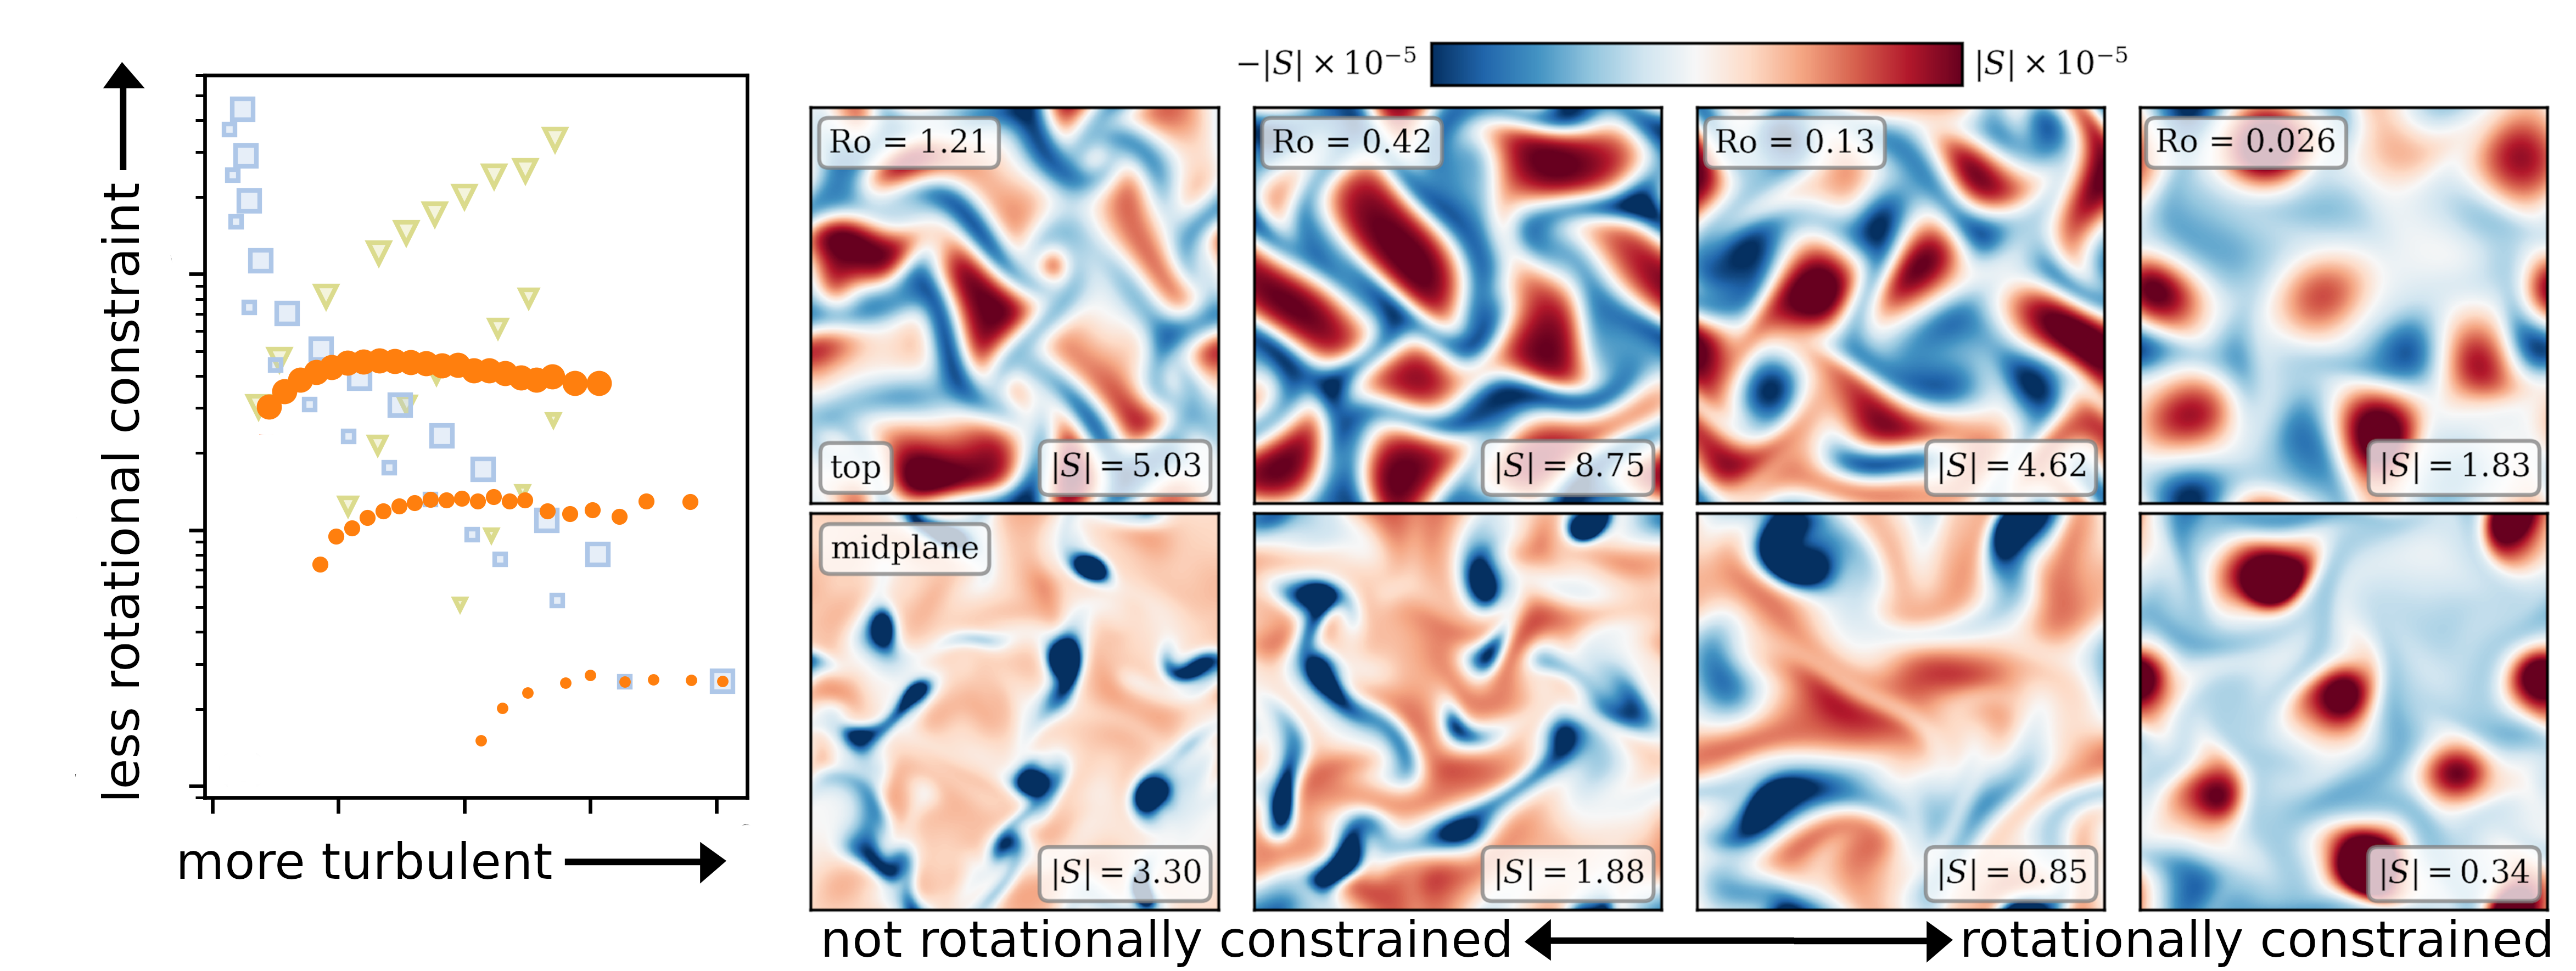
\includegraphics[width=\textwidth]{./figs/rossby_plot.png}
    \caption{(left, Fig 1b of \citet{anders&all2019}) The Rossby number, Ro, is difficult to predict as a function of the Rayleigh number, Ra, in rotating convection.
	Along traditional ``convective Rossby number'' (green) paths through parameter space, Ro increases as a function of Ra, and along constant supercriticality paths (blue) it decreases.
	Walking along paths along the newly discovered ``predictive Rossby number'' (orange) seems to hold the value of Ro, and thus the degree of rotational constraint, constant.
	(right eight panels, Fig. 2 of \citet{anders&all2019}) As you decrease the Rossby number (from left to right), traditional granular convective patterns give way to quasi-two-dimensional vortical columns of convection with very little difference between the top of the atmosphere and the atmospheric midplane (top row vs. bottom row).
	It is clear to see that changing the Rossby number massively effects convective dynamics and therefore choosing a value of Ro that reflects the astrophysical object of interest being studied (e.g., the Sun) is crucial.
	\label{fig:rossby_plot} }
\end{figure*}


Task B will build naturally both on the work of task A and on the low mach number, fully compressible work I studied during my graduate career \citep{anders&brown2017, anders&all2019}.
This task will have two phases: a study of rotating convection and a study of magnetoconvection.
In all cases, I am particularly interested with the manner in which convective motions interact with and transport momentum in the presence of stable layer.
Thus, these simulations will include an upper convective region and a lower stable region, introducing a new dimension to the parameter space: the stiffness of the convective-radiative boundary \citep[or, whether or not convective motions can penetrate the stable region, as in][]{couston&all2017}.
Most modern convective simulations study dynamics in the regime of low stiffness, but if low Mach number flows in the Sun impact a very stable radiative layer, it is quite possible that solar downflows feel a stiff boundary.
Thus, I will study the differences in vector transport achieved at low and high stiffness.

\subsubsection{Task B.1: Transport of angular momentum by convection}
The simulation setup here will be precisely the same as in Task A.1, but where time-dependent convection is studied instead of thermals.
During my graduate career, I indentified how to study low mach number, fully compressible convection \citep{anders&brown2017} and how to set the output degree of rotational constraint (Rossby, Ro) using input values \citep[][and Fig. \ref{fig:rossby_plot}]{anders&all2019}.
As a result, performing the same sweep of parameter space as in Task A.1 should be straightforward.
These simulations will aim to determine how stiff and squishy interfaces with stable regions affect transport of angular momentum in a time-averaged sense.
In the Sun, the interior stable layer rotates uniformly while the convection zone rotates differentially, and thus one desired outcome of this work is to find which parameter space regime either transmits no angular momentum to the stable layer, or a regime where the transmission of angular momentum is constant as a function of latitude (is this right? need to think).
Finding this regime will help us identify the flow regime of the deep solar convection zone and understand why giant cells are not driven there.

\subsubsection{Task B.2: Transport of magnetic fields by convection}
This task is similar to Task A.2, but is less straightforward than Task B.1.
In the case of magnetoconvection, it is not yet known how to precisely control the output value of (plasma beta? What's the right value?).
Thus, the first step of Task B.2 will be to determine how the (output value) of the flows is set by the Chandrasekhar number and the Rayleigh number.
Once this is determined, a simple sweep through parameter space, as in task A.2 and B.1 will be performed.
Once again, the primary question I aim to answer is how convective motions transport magnetic field across a stable region.
\citet{tobias&all1998} showed that when the interface is squishy, convective motions can effectively pump magnetic fields across it.
It is unclear if the same is true for stiff interfaces, and in such a case it is important to understand if the magnetic field is pumped into the layer or remains in the convection zone.
The base of the solar convection zone -- the tachocline -- is not only a boundary region of a convecting and stable region, but is also a region with a large amount of shear where the solar differential rotation gives way to the uniformly rotating interior.
The shearing motions in this region are thought to be crucial for the solar dynamo, and so understanding which regimes allow for magnetic field transport into that region will be crucial for better understanding dynamos in solar-type stars.


\subsection{Task C: Dynamo simulations in proper solar or stellar regimes}
\label{sct:global_models}
The experiments laid out in Tasks A \& B foundational for the capstone projects of my postdoctoral studies: global simulations of rotating magnetoconvection in spherical domains, or dynamo simulations.
The tools to perform these simulations in Dedalus already exist (TODO: see pretty figure and X references), but will be more robust by the time this phase of my project begins.
This task will likewise have two phases, both of which will be informed by the results of tasks A and B.

\subsubsection{Task C.1: Creating tools to accelerate the evolution of mean angular momentum and magnetic field profiles}
One major barrier to performing global dynamo simulations is that they are costly.
The wall time of state-of-the-art simulations which display interesting dynamo or rotational statistics are best estimated to take timescales of months.
Some of these costs are unavoidable: highly resolved turbulent simulations necessarily take small timesteps, and therefore results come slowly.
However, some of the expense of these simulations is often time wasted.
System structure and mean flows, such as differential rotation, often converge over timescales which are much larger than convective overturn timescales.
For example, the thermal structure of the Sun is thought to evolve over its Kelvin-Helmholtz timescale of $10^7$ years, which is significantly longer than its convective overturn time of five minutes at the solar surface.
As we strive to push simulations into increasingly realistic regimes, the separation between these timescales becomes more extreme (eventually approaching that of the Sun), and it can take unaffordable numbers of overturn times for atmospheric structure and mean flows to evolve.
These long evolutionary timescales are a problem, because they limit our ability to understand the dynamical nature of convection in stars.

During my graduate career, I studied a mechanism for accelerating the long thermal relaxation timescale in convective systems.
This mechanism is published for Boussinesq convection \citep{anders&all2018} and has been adapated to stratified, compressible convection in plane-parallel systems within our research group to be used in forthcoming work.
At even modest values of the Rayleigh number, we found that we could reach a converged state using an order of magnitude fewer computational resources than when waiting for a standard thermal relaxation timescale.
These speedups make achieving thermal relaxation in state-of-the-art simulations feasible.

During my postdoctoral studies, I will extend my accelerated evolution (AE) method to the transport of angular momentum and magnetism in dynamo simulations.
The development of this extension will be grounded in an understanding of the transport mechanisms of these quantities which I will gain in tasks A and B.
In essence, the procedure described in \citet{ander&all2018} is one which allows the user to take timesteps for the mean state and the mean flows which are much larger than those allowed by convection.
As I did in \citet{anders&all2018}, I will verify that this method produces the same results as a long relaxation in modest parameter regimes to build trust in the method.
Once developed, this tool will of course be made publicly available (as described in the part of the proposal where I describe these things).

\subsubsection{Task C.2: Relaxed simulations of the solar dynamo}
Global simulations are expensive (on the order of $10^6$ cpu-hours per run), and so only a select few of these simulations can be conducted.
I will study simulations of the interior solar convection zone in the low-Ro regime, as some results suggest may be appropriate, and in the regime where both magnetism and fluid advection are relatively equally balanced (TODO: Is this the right regime and if not how do we determine it?)
Using the tool developed in task C.1, I will accelerate the evolution of these simulations in order to study their result with well-developed mean flows and relaxed thermodynamic mean profiles.
I hope to find that in the parameter regimes that we expect the Sun to exist (from observations, the work of others, and the work in tasks A and B), the global simulations develop a solar-like differential rotation, a sharp tachocline, and a solar-like dynamo.

These simulations will be largely aimed at helping solve the convective conundrum, but the accelerated evolution tools which will be developed and tested here could have great benefits for asteroseismic research.
New research is beginning to couple three-dimensional, global simulations with 1-dimensional stellar structure tools in order to more accurately produce stellar structure profiles \citep{jorgensen&weiss2019}.
The fast equilibration of angular momentum and thermal profiles described here is essentially equivalent to taking timesteps which superstep the convective motions, similar to those taken in any one-dimensional stellar structure model.
These techniques presented here would therefore allow the coupling of 1-dimensional stellar structure codes with realistic statistics from three-dimensional convection to create converged stellar profiles, including latitudinal variations like differential rotation.
While the linking of these disparate techniques is beyond the scope of my postdoctoral research, I will design the code with this eventual use case in mind such that future implementation of such a method -- by myself or others -- is fairly straightforward.

\section{Collaborative studies at CIERA and Northwestern University}
\label{sct:northwestern}
Northwestern university, and specifically the CIERA institue, is the perfect location for me to carry out the work proposed here.
Dr. Daniel Lecoanet, who will be my primary advisor and collaborator, will be arriving in the Fall of 2020, and I would be arriving concurrently.
As one of the code's founders, Dr. Lecoanet an expert in Dedalus and his past work on thermals \citep{lecoanet&jeevanjee2019, tarshis&all2018}, convection \citep{lecoanet&quataert2013, lecoanet&all2014, couston&all2017}, rotating convection \citep{couston&all2019}, and global simulations \citep{lecoanet&all2018} make him excellently qualified to advise me on the projects proposed here.
Furthermore, I have already published one paper in collaboration with Dr. Lecoanet and so there would be no lag in figuring out a successful collaborative and professional relationship upon my arrival.
In addition to Dr. Lecoanet, Dr. Yoram Lithwick would be an excellent partner for collaboration due to his past work on rotating convection \citep{BDLithwick2014} and his continuing collaborations on studying careful and numerical problems in fluid disks \citep{LDLithwick2019} and planetary systems \citep{hadden&lithwick2018} would provide excellent opportunities for collaboration.
Despite working on disparate applications, I also anticipate that the work proposed here will benefit from fruitful conversations with other members of the institute, such as Dr. Sasha Tchekhovskoy, whose background in general relativistic MHD simulations is extensive \citep[as in e.g.,][]{tchekhovskoy&bromberg2016}.

In addition to the collaborative opportunities available at CIERA, being housed at CIERA will provide me with access to high performance computing resources which will be crucial to the work here.
The small in-house 252-core CIERA cluster will enable small-scale exploratory work that will assist in developing my understanding of the bounds of parameter space.
Northwestern's larger 11,800-core Quest supercomputer has sufficient resources for most of the 3D simulations presented in this work, all of which should be performable on 1024 cores.
In order to increase my access to computational resources and to allow for larger scale runs, I will leverage my AAPF fellowship and apply for time on NSF XSEDE resources such as Stampede2, Comet, or Bridges.

Furthermore, in addition to the focused educational and outreach projects below, being centered at CIERA will provide me with numerous small scale opportunities to participate in public outreach.
CIERA's Astronomy on Tap program as well as its CIERA Astronomer Evenings provide bite-sized and accessible ways to interact with the public.
Dearborn Observatory's observation tours are very similar to the public open houses I helped host at CU Boulder's Sommers-Bausch observatory.
The state-of-the-art Adler planetarium also provides similar opportunities such as its \emph{`Scopes in the City} program or its Space Visualization Lab astronomy conversations.


\section{Broader Impacts: Supporting the growth of young career scientists as educators and individuals}
\label{sct:outreach}
Through the implementation of two small programs which leverage collaborations with existing programs or institutes at Northwestern, I aim to support diverse young career students at the university level with a network of supportive peers while also creating meaningful opportunities for them to develop as educators and professionals.
Their development will also result in the teaching of authentic inquiry at the high school level, thereby serving the broader community.

Side note: NSF language that is applicable and that I need to work in here: ``Such outcomes include, but are not limited to: full participation of women, persons with disabilities, and underrepresented minorities in science, technology, engineering, and mathematics (STEM); improved STEM education and educator development at any level; increased public scientific literacy and public engagement with science and technology; ...development of a diverse, globally competitive STEM workforce...''



\subsection{Teaching and Outreach: Preparing early career scientists as teachers}
During my graduate career I twice participated in the University of California Santa Cruz's Institute for Scientist and Engineering Educators Professional Development Program (UCSC ISEE PDP), an NSF-funded program which teaches early career scientists the basics of teaching pedagogy in the context of developing and teaching an authentic STEM inquiry activity.
While the PDP is open to graduate students, postdocs, and faculty members at all universities in the US, in general only a small group of individuals from any one institution can participate in a given year.
My experiences in this program helped me gain confidence in knowing that teaching is an important piece of my future career, and laid the foundation of my knowledge of what it means to be a teacher and how teaching can be informed by scientific literature.
I propose to develop a one-semester course for graduate students and senior undergraduate students which teaches the basics of teaching pedagogy and culminates in authentic teaching experiences in either high school classrooms.
I will spend 10-15\% of my time during my first year as a postdoctoral researcher developing and establishing the infrastructure for this course, then I plan to teach the course in the Fall of 2021 and 2022.
Over the course of Spring and Summer I will iterate and improve on my course materials based on student performance and feedback, and in Spring and Summer of 2023 I will ensure that the course materials are made available to Northwestern faculty before my fellowship ends.

The culminating project of this course will be an authentic teaching experience for the students, something which many young scientists do not have in their undergraduate or graduate preparation.
In order to coordinate these teaching experiences, I will leverage connections with the CIERA-based and NSF-funded \href{http://gk12.ciera.northwestern.edu/}{Reach for the Stars} program, a GK-12 program.
Reach for the Stars is a selective program which offers a small number of graduate students an opportunity to spend 10-15 hours per week in the high school classroom leading young students through authentic scientific inquiry experiences while teaching those students how to think computationally and use computational tools.
Exposing young students to authentic scientific inquiry activities is crucial because students not only learn STEM content but also participate in using STEM practices, such as creating hypotheses or designing and carrying out investigations.
Reach for the Stars' \href{https://avault.github.io/}{Vault} program does an excellent job of providing a space for students to participate in these practices.
These practices are often not explicitly taught, and this can make it difficult for scientists to communicate their processes.
Fortunately modern literature \citep[e.g.,][]{dasgupta&all2014} is breaking down struggles that students face in learning the \emph{practices} of science, which can help guide our design of in-the-classroom activities which focus on teaching these practices.
This class will complement Reach for the Stars by providing an opportunity for professional development to a larger number of students which is overall a smaller time commitment and less selective while still offering the students an opportunity for professional growth and impactful outreach.

One guiding principle of proper course design is backwards design \citep{wiggins&mctighe1998}, which is \emph{logically} foward, but \emph{in practice} backwards from how many courses are designed.
In essence backward design states that you start with the learning outcomes you want your students to achieve, then you design careful assessments to determine whether or not those learning goals were met, and \emph{only then} do you design the course content.
An understanding of the backwards design process is one of the learning goals I have for students who take this course, but I will also use these principles in the design of this course.
Since the culminating project of the course for the students will be to teach a topic in the high school classroom, I will rely on the high school teachers to provide us with a learning outcome that fits their curriculum, and it will then be the role of the students to work backwards from that goal in the design of their inquiry activity.

I will design specific tasks that students will undergo during Fall 2020 - Spring 2021, but in general the course will cover four broad topics, each of which has been heavily influenced by the groundwork and structure of ISEE's PDP program.
In the first unit, students will learn about backwards design in the context of inquiry activities, including specific care about how to set both content and practice learning goals for their students and different activity structures which leave space for authentic inquiry while also ensuring students arrive at those learning outcomes.
In the second unit, we will discuss different types of assessments, when these types of assessments are appropriate, how to create honest and fair rubrics, and how to align a rubric with an assessment.
In the third unit, we will discuss equity and inclusion, including published research regarding the effects that inequities have on students, and discuss how to design inclusive activities with multiple pathways for success so that all learners can achieve the learning goals.
In the fourst unit, students will experience the culmination of the work that they have done through the semester by teaching in the college classroom, and then we will discuss methods for iterating on course design in order to improve it for the future.

This course will provide young career scientists with a foundation in how to teach, things to consider while teaching, and will also give them an opportunity to try out some teaching practices in a fairly low-stakes setting.
The students will be graded on their thoughtful creation, analysis, and reflection on their course design rather than on the specific teaching outcomes of their activity.
Furthermore, the culminating project for each group of students is by definition an outreach activity: the students will go into nearby high school classrooms, engage with young students about science, provide authentic and inclusive experiences in STEM, and in doing so broadly impact the nearby community.

\subsection{Inreach: Peer mentorship for the retention of undergraduates and early graduate students}
The path to a career in the US STEM workforce is a leaky pipeline.
Data show that in particular, underrepresented minority groups and women pursue careers in STEM fields at a rate which is disproportionately low compared to the share of the total population that those groups constitute \citep{corbett&hill2015, nsf2019}.
While a great deal of focus is rightly placed on changing the career outlooks of these groups before the collegiate level, the pipeline continues to leak at the baccalaureate and post-baccalaureate levels, and underrepresentation becomes more severe.

Mentoring has long been known to play a significant role in increasing retention and helping new departmental members acclimate to the department climate \citep{hunt&michael1983}.
Establishing robust mentoring programs based on evidence and knowledge of the recent literature in mentorship \citep[as in e.g.,][]{crisp&all2009, crisp&all2017} can be one critical component of helping broaden participation of underrepresented and marginalized groups in the STEM workforce.
During my graduate studies, I spent three years working with the University of Colorado's CU-STARs group.
CU-STARs is a combined ``outreach'' and ``inreach'' program with the dual aims of increasing STEM engagement for students at underserved, rural schools across Colorado while decreasing attrition of underrepresented groups in CU Boulder's Astrophysical and Planetary Sciences department.
One of my many roles as a graduate student administrator in this group was to mentor undergraduate students, although we were never formally trained in mentoring, nor did we have a robust mentoring structure in place to support mentors and mentees alike.

During my years at Northwestern, I propose to work with the experts in Northwestern's \href{https://www.northwestern.edu/searle/index.html}{Searle Center for Advanced Teaching and Learning} to develop peer mentoring programs within Northwestern University's applied math department and the department of physics and astrophysics.
The goal of this program will be to connect students with peers who are slightly more advanced in their careers.
For example, entering undergraduate mentees would connect with junior or senior undergraduates in the field; senior undergraduates mentees could connect with young graduate student mentors; young graduate student mentees could connect with senior graduate students; and senior graduate students could connect with postdoctoral students.
In general, we would aim to connect young scientists who are still at a close enough level of their career to fully understand the experiences of one another to give young students advice and provide them with a professional support network.

I will lay the groundwork for this organization in my first year at Northwestern and plan to roll it out in my second year, starting in the fall of 2021.
My first year will be spent collaborating with my hosting department, as well as other very related departments like the department of Physics and Astronomy, in order to gain university buy-in at the faculty level to ensure that this program will continue to run after I leave.
I will also collaborate with the Searle Center and others to ensure that I establish proper training for mentees.
Furthermore, I will begin searching at the University level for sustainable \href{https://www.northwestern.edu/studentorgs/org-officers/funding/index.html}{funding} so that this organization can support the purchasing of coffee for mentor meetings.
I will also aim to secure enough funding for the organization to buy snacks for infrequent social meetings.

\subsection{Personal career growth and development}
Need to write this in more words, but basically my past experiences have shown me that I truly enjoy both research and teaching.
Setting up these programs will allow me to grow in the teaching / service aspect of an academic career while also giving younger students a taste of that aspect of this career path so that they can help decide if they like it.



\section{Summary and Perspectives}
\label{sct:summary}
TODO

\bibliographystyle{apj}
\bibliography{biblio}
\end{document}
